\section{Results Consideration}
\label{sec:Results}
\subsection{Output of GA for tested lamps}

The results of genetic algorithm are shown in tables~\ref{tab:onesideLamps} and \ref{tab:twosideLamps}. The results should be considered as solutions close to optimum specified by the fitness function. Genetic algorithms are capable of multi parametric optimization, but they are also unable to give exact solutions (\cite{Zelinka2009}, \cite{Fogel2006}). The perfect optimum must be searched by some method with tighter limits around found optimum. Very often is used an combination of genetic algorithm to get close to optimum and then some other stochastic or deterministic algorithm to find the perfect optimum.

The algorithm found different solution during the testing, that fulfill defined constraints. This is normal behavior of the algorithm. If more than one solution exist with close maximums of the fitness, then the algorithm randomly found one of them. The designers can have some preferences. For example they might prefer that the pillars highs cannot be more than 10~m or that the distances between the pillars must be as far as possible an so on. These preferences must be then somehow included to set limits of searched values or in the composition of the fitness function. Authors set pretty lose limits, therefore there are more than one close to optimal solution for some types of the lamps. Other possible solutions are not presented in table~\ref{tab:onesideLamps} nor in table~\ref{tab:twosideLamps}.
 
\begin{table}[htb]
	\renewcommand{\arraystretch}{1.3}
	\caption{Results for one side lamp placement}
 	\label{tab:onesideLamps}
	\centering
  \begin{tabular}{ l | c | c | c | c | c | c | c }
    \hline
    \textbf{Type} & $D_X$ & $D_Y$ & $Z$ & $\alpha$ & $\overline{E}$ & $E_{min}$ & $\overline{E}_o$\\ 
    & (m) & (m) & (m) & ($^\circ$) & (lx) & (lx) & (lx)\\ \hline
    ATOS 70W A1 & 39.8 & 0.67 & 6.22 & 3.15 & 8.14 & 1.31 & 7.40\\ \hline
    ATOS 70W A2 & 41.8 & -0.73 & 6.54 & 2.43 & 8.13 & 1.42 & 7.25\\ \hline
    ATOS 70W A3 & 44.9 & -1.69 & 6.47 & 3.34 & 8.15 & 1.36 & 6.86\\ \hline
    ATOS 70W A4 & 47.9 & -0.41 & 6.97 & 3.59 & 8.14 & 1.36 & 6.72\\ \hline\hline
    ATOS 70W B1 & 36.8 & 0.09 & 6.86 & 2.77 & 8.13 & 1.31 & 7.70\\ \hline
    ATOS 70W B2 & 41.1 & -1.29 & 7.28 & 1.69 & 8.14 & 1.34 & 7.17\\ \hline
    ATOS 70W B3 & 45.4 & -1.40 & 7.76 & 1.29 & 8.14 & 1.55 & 6.84\\ \hline
    ATOS 70W B4 & 49.5 & -1.59 & 7.69 & 2.54 & 8.13 & 1.72 & 6.76\\ \hline\hline
    ATOS 70W C1 & 37.6 & -0.60 & 6.23 & 6.57 & 8.13 & 1.38 & 7.65\\ \hline
    ATOS 70W C2 & 41.14 & -0.59 & 6.72 & 1.86 & 8.14 & 1.50 & 7.30\\ \hline
    ATOS 70W C3 & 45.1 & -0.75 & 6.56 & 5.49 & 8.14 & 1.31 & 6.91\\ \hline
    ATOS 70W C4 & 48.0 & 0.03 & 6.85 & 6.70 & 8.14 & 1.36 & 6.92\\ \hline
  \end{tabular}
\end{table}

\begin{table}[htb]
	\renewcommand{\arraystretch}{1.3}
	\caption{Results for two sides lamp placement}
 	\label{tab:twosideLamps}
	\centering
  \begin{tabular}{ l | c | c | c | c | c | c | c }
    \hline
    \textbf{Type} & $D_X$ & $D_Y$ & $Z$ & $\alpha$ & $\overline{E}$ & $E_{min}$ & $\overline{E}_o$\\ 
    & (m) & (m) & (m) & ($^\circ$) & (lx) & (lx) & (lx)\\ \hline
    ATOS 70W A1 & 39.2 & -0.21 & 6.24 & 3.85 & 8.14 & 1.32 & 7.55 \\ \hline
    ATOS 70W A2 & 40.9 & -0.58 & 6.19 & 7.60 & 8.13 & 1.31 & 7.40\\ \hline
    ATOS 70W A3 & 44.5 & -0.90 & 6.54 & 5.40 & 8.13 & 1.35 & 6.98\\ \hline
    ATOS 70W A4 & 45.8 & -1.42 & 6.45 & 10.51 & 8.13 & 1.42 & 6.82\\ \hline\hline
    ATOS 70W B1 & 36.8 & 0.07 & 6.87 & 3.25 & 8.13 & 1.34 & 7.70\\ \hline
    ATOS 70W B2 & 41.0 & -0.46 & 7.25 & 0.81 & 8.13 & 1.35 & 7.41\\ \hline
    ATOS 70W B3 & 43.6 & -1.11 & 7.53 & 5.24 & 8.13 & 1.61 & 7.06\\ \hline
    ATOS 70W B4 & 48.51 & -1.49 & 7.34 & 8.76 & 8.13 & 1.30 & 6.73\\ \hline\hline
    ATOS 70W C1 & 37.4 & -0.45 & 6.73 & 0.55 & 8.14 & 1.60 & 7.64\\ \hline
    ATOS 70W C2 & 41.1 & -1.28 & 6.55 & 3.09 & 8.14 & 1.34 & 7.18\\ \hline
    ATOS 70W C3 & 46.0 & -0.76 & 6.95 & 1.03 & 8.13 & 1.38 & 6.68\\ \hline
    ATOS 70W C4 & 49.8 & -0.14 & 7.09 & 1.90 & 8.14 & 1.32 & 6.62\\ \hline
  \end{tabular}
\end{table}

\subsection{Example of specific result for ATOS 70 W A1}
The result for the lamp ATOS 70 W A1 is discussed in this chapter. The output parameters of the algorithm can be found in the first row of the tables~\ref{tab:onesideLamps} and~\ref{tab:twosideLamps}. The count of tested points in control area were decreased to 960 for better visualization in figures~\ref{fig:exampleOS} and~\ref{fig:exampleTS}. The distances between points is then 0.5~m in the visualizations.

The change of the fitness function during each generation is  presented in figures~\ref{fig:exampleOSFit} and~\ref{fig:exampleTSFit}. The fitness function in case of one side lamp placement has the most typical shape for a most of the done tests. The algorithm found good solution very fast on the beginning of the optimization and then the growth of the fitness function slew down. The shape in figure~\ref{fig:exampleTSFit} did not appeared too much. The faster growth at older generations was usually caused by poor initial solutions in very first generations. It was pretty possible event, because the first solutions in populations were always chosen randomly. However the algorithm is capable found good solution due to mutation presence in next generations.


\begin{figure}[t]
        \centering
        \subfloat[Fitness function during the optimization \label{fig:exampleOSFit}]{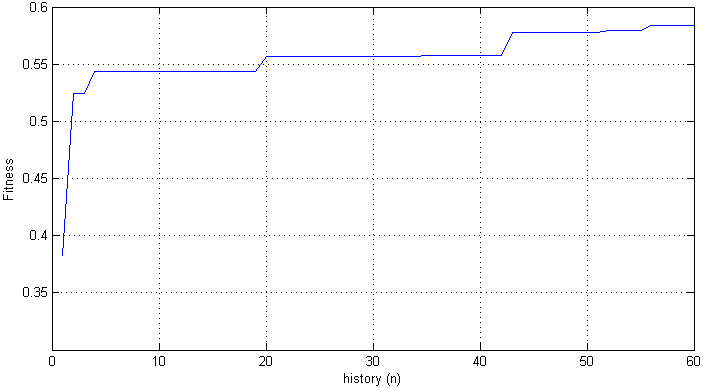
\includegraphics[width=\columnwidth]{GrafyOS_Fit}}\\
        \subfloat[Color map represents lighting on the road, best offspring]{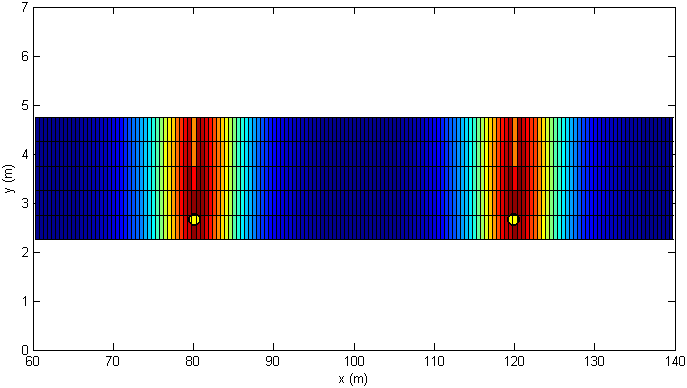
\includegraphics[width=\columnwidth]{GrafyOS_Fill}}\\
        \subfloat[Lighting on the road, best offspring]{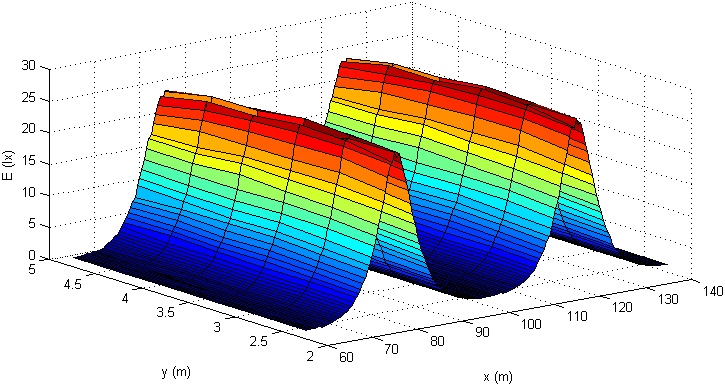
\includegraphics[width=\columnwidth]{GrafyOS_3D}}
        \caption{Example of result of lamp ATOS~70~W~A1 for one side placement}
        \label{fig:exampleOS}
\end{figure}

\begin{figure}[t]

        \centering
        \subfloat[Fitness function during the optimization \label{fig:exampleTSFit}]{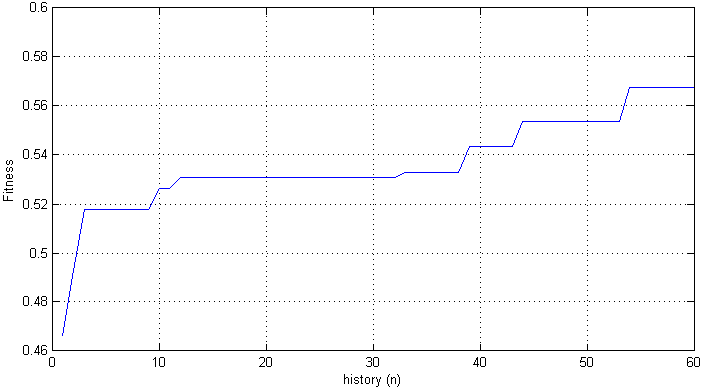
\includegraphics[width=\columnwidth]{GrafyTS_Fit}}\\
        \subfloat[Color map represents lighting on the road, best offspring]{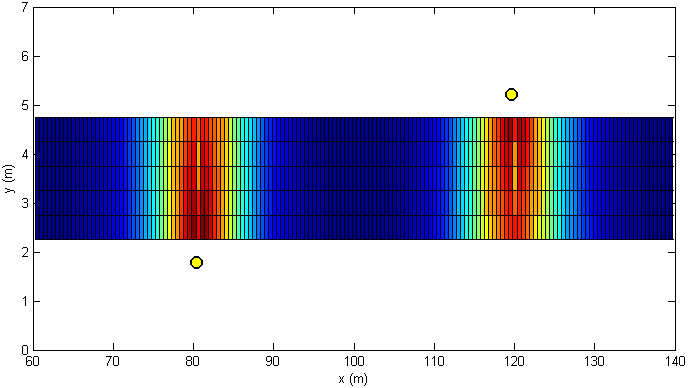
\includegraphics[width=\columnwidth]{GrafyTS_Fill}}\\
        \subfloat[Lighting on the road, best offspring]{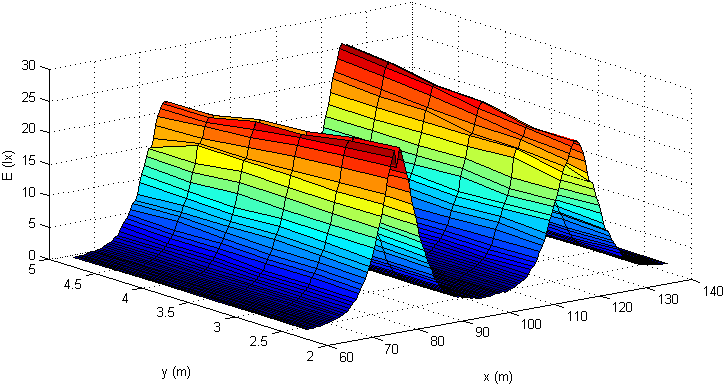
\includegraphics[width=\columnwidth]{GrafyTS_3D}}
        \caption{Example of result of lamp ATOS~70~W~A1 for two side placement}
				\label{fig:exampleTS}
\end{figure}

\subsection{Comparing Results with DIALux Output}

A portion of the results were compared with data obtained from an identical situation simulated in DIALux software, where a street project has been created using luminaires Atos A1 on one side of the road. Horizontal illuminances at road surface level were calculated by DIALux according to~\cite{CSN_EN_13201-3} as depicted in figure~\ref{fig:Standard13210-3} and the output in lux can be found in table~\ref{tab:DialuxOneSideLamps} with applied maintenance factor $MF=0.79$ (see equation~\ref{eq:MFSpecific}).

\begin{figure}[htb]
  \centering
  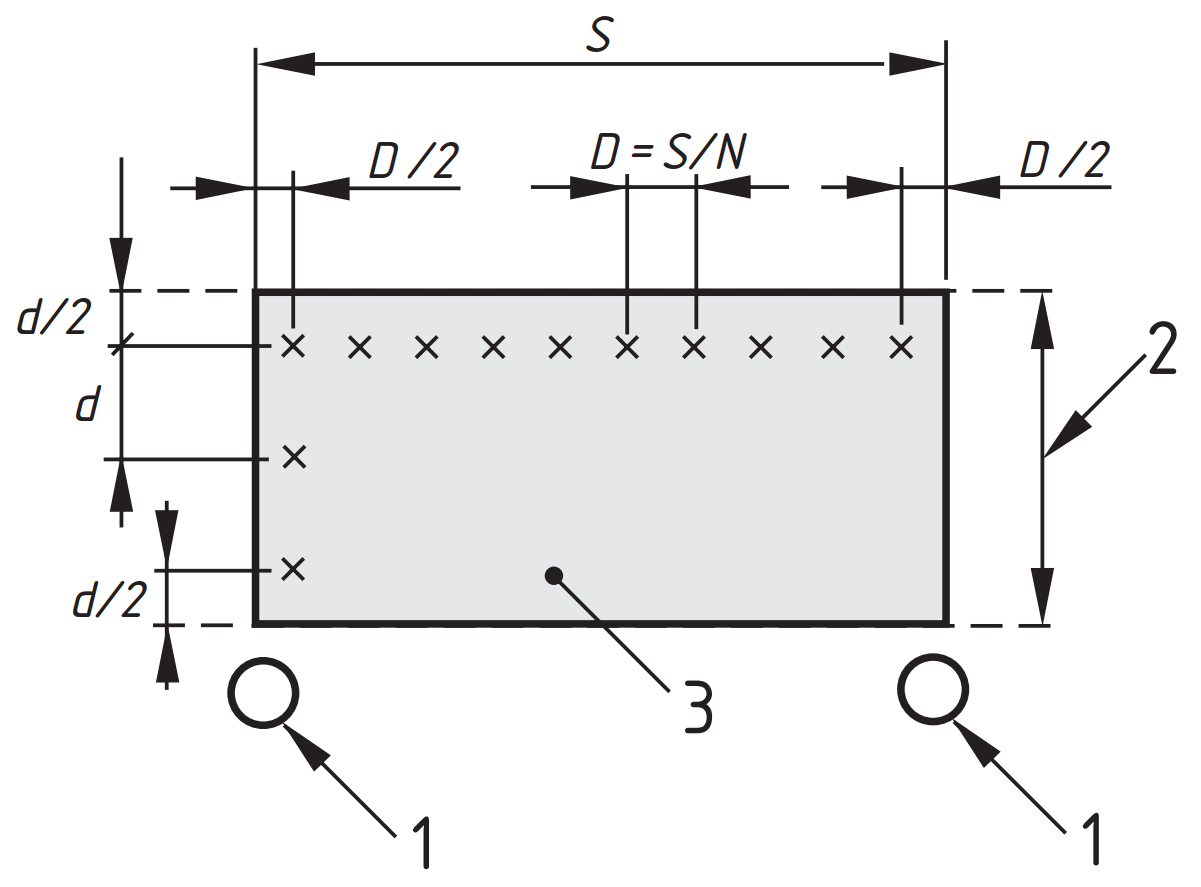
\includegraphics[width=0.8\columnwidth]{13201-3_points}
	\begin{description}
		\item[1] luminaire
		\item[2] width of relevant area $W_{r}$
		\item[3] field of calculation
		\item[x] denotes lines of calculation points in the transverse and longitudinal directions
	\end{description}
	\caption{Calculation points on relevant area \cite{CSN_EN_13201-3}}
  \label{fig:Standard13210-3}
\end{figure}

\begin{table}[htb]
	\renewcommand{\arraystretch}{1.3}
	\caption{DIALux calculated horizontal design illuminances in lux}
 	\label{tab:DialuxOneSideLamps}
	\centering
  \begin{tabular}{ l || c | c | c | c | c | c | c }
    \hline
    \textbf{(m)} & 1.421 & 4.264 & 7.107 & 9.950 & 12.793 & 15.636 & 18.479\\ \hline \hline
    2.5 & 24.17 & 16.54 & 9.5 & 4.77 & 2.91 & 1.98 & 1.64\\ \hline
		1.5 & 25.45 & 15.27 & 8.59 & 4.13 & 2.61 & 1.78 & 1.49\\ \hline
		0.5 & 25.45 & 15.27 & 7.82 & 3.72 & 2.35 & 1.63 & 1.36\\ \hline \hline \hline
		\textbf{(m)} & 21.321 & 24.164 & 27.001 & 29.850 & 32.693 & 35.536 & 38.379\\ \hline \hline
		2.5 & 1.64 & 1.98 & 2.91 & 4.77 & 9.5 & 16.54 & 24.17\\ \hline
		1.5 & 1.49 & 1.78 & 2.61 & 4.13 & 8.59 & 15.27 & 25.45\\ \hline
		0.5 & 1.36 & 1.63 & 2.35 & 3.72 & 7.82 & 15.27 & 25.45\\ \hline
  \end{tabular}
\end{table}

According to standard~\cite{CSN_EN_13201-3} calculation points shall not be spaced in the longitudinal directions more than 3 m from each other, so 14 calculation points were used during calculations of DIALux instead of 10 depicted in figure~\ref{fig:Standard13210-3}.

\begin{table}[htb]
	\renewcommand{\arraystretch}{1.3}
	\caption{DIALux input data and illuminances}
 	\label{tab:DialuxIlluminances}
	\centering
  \begin{tabular}{ c | c | c | c | c | c | c }
    \hline
    \textbf{Type} & $D_X$ & $D_Y$ & $Z$ & $\alpha$ & $\overline{E}$ & $E_{min}$\\
		& (m) & (m) & (m) & ($^\circ$) & (lx) & (lx)\\ \hline
    ATOS 70W A1 & 39.8 & 0.67 & 6.22 & 3.1 & 8.52 & 1.36\\ \hline
  \end{tabular}
\end{table}

Comparing the first data row of table~\ref{tab:onesideLamps} and table~\ref{tab:DialuxIlluminances} similar values of illuminances $\overline{E}$ and $E_{min}$ can be found calculated by both DIALux and the methods used in the genetic algorithm. Small differences for the Atos 70 W A1 used in the comparison could be caused by a vast difference in the amount of calculation points.